% Chapter 4

\chapter{Knowledge Compilation} % Chapter title

\label{ch:compilation} % For referencing the chapter elsewhere, use \autoref{ch:examples}

%----------------------------------------------------------------------------------------

The study of Logic Circuits (LCs) in the field of Circuit Theory (CT)
predates the creation of Logic Programming languages and other topics
covered in this thesis. In greater detail, Logic Circuits are integral
components in one of the most fundamental theorems of computer theory: the
Cook-Levin Theorem, which states that \textsc{SAT} is
\textsc{NP}-complete \citep{Cook_1971, levin1973universal}.
Moreover, the expressiveness of these \textsc{SAT}-like problems in
modeling real-world scenarios, such as Enumerative Combinatorial
problems \citep{valiant1979189} or interdisciplinary
applications (e.g., Bioinformatics \citep{bacchus2021maximum}),
motivates the development of efficient structures and algorithms
to solve these problems.

Therefore, with the preliminary definitions of PASP in
the previous chapter \ref{ch:pasp}, we have sufficient
motivation to proceed with a formal definition of Logic Circuits,
needed to perform the Knowledge Compilation for PASP proposed in this work.
We define the Negation Normal Form Language (NNF), a language capable of
unifying well-known succinct data structures for representing
Boolean formulas, such as Binary Decision Diagrams (BDDs),
Sentential Decision Diagrams (SDDs), and Decomposable Negation Normal Form
(DNNFs) \citep{Darwiche_2002, darwiche2011sdd}.

%----------------------------------------------------------------------------------------


\section{Negation Normal Form Language}

We begin with the formal definition of the NNF, a language
capable of unifying well-known efficient data structures for
representing Boolean formulas, such as CNF, DNF, OBDD, DNNF,
SDD, and MODS \citep{Darwiche_2002}.

The notation and definitions in this section are heavily
influenced by the work of \citep{Darwiche_2002,
darwiche2011sdd} and \citep{kisa2014probabilistic}.

\begin{definition}[Negation Normal Form Language]
    Let $V$ be a set of propositional variables. Then, we say
    that a sentence is in $\mathrm{NNF}_V$ if it is a \textit{rooted}
    Direct Acyclic Graph (DAG) where each leaf is labeled as one of
    the following:

    \begin{itemize}
        \item \textit{True} or \textit{False}, or
        \item $X$ or $\neg X$, with $X \in V$;
    \end{itemize}

    and each internal node is labeled with $\land$ or $\lor$ and
    can have arbitrarily many children.

    The \textit{size} of a sentence $\Sigma$ in
    $\mathrm{NNF}_V$, denoted $|\Sigma|$, is the number of edges
    of its DAG; and the \textit{height} is the depth, the
    longest path from the root to a leaf of the DAG.
\end{definition}

An important note is that the NNF language is not a
\textit{target compilation} language (unless $P \ne NP$)
\citep{papadimitriou2003computational}, as it is not
tractable enough to permit a non-trivial set of polynomial
queries \citep{Darwiche_2002}. However, many of
its subsets are target compilation languages, as they impose
structural constraints that enable succinct representations
and allow for efficient algorithms to perform queries on them.

Another important class of languages is called
\textit{representation languages}, which we loosely define as
human-interpretable languages \citep{Darwiche_2002}. Both
CNFs and Horn Clauses (or Rules) are examples of
representation languages.

\subsection{Flat Normal Form Language}

In addition to our earlier definitions of \textit{target compilation} and
\textit{representation} languages, we can also categorize
NNFs subsets as \textit{flat} or \textit{nested} languages.
We describe the former first as follows:

\begin{definition}[Flat Normal Form Language]
    A \textit{flat} NNF is an NNF that satisfies the
    following three properties:

    \begin{itemize}
        \item \textbf{Flatness:} The height of the sentence's
        DAG is at most 2;
        \item \textbf{Simple-Conjunction:} All conjunction nodes
        (\textbf{and}-nodes) have children that are leaves sharing no
        variables; and
        \item \textbf{Simple-Disjunction:} All disjunction nodes
        (\textbf{or}-nodes) have children that are leaves sharing no
        variables.
    \end{itemize}

    Note that since the leaves are either literals or
    constants, \textbf{and}-nodes of a flat NNF are
    conjunctive clauses. Similarly, the \textbf{or}-nodes of a
    flat NNF are disjunctive clauses.

    We define $f-\mathrm{NNF}$ as the subset of NNFs that
    satisfies the \textit{flatness} property.
\end{definition}

Figure \ref{fig:cnf_dnf} shows examples of a CNF and a
DNF, respectively, using the NNF language. Note that
Figure \ref{fig:cnf} satisfies both the \textit{flatness} and
\textit{simple-disjunction} properties, while Figure
\ref{fig:dnf} satisfies the \textit{flatness} and
\textit{simple-conjunction} properties.

\begin{figure}[bth]
    \centering
    \begin{subfigure}[b]{.45\linewidth}
        \centering
        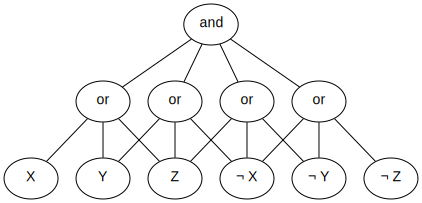
\includegraphics[width=\linewidth]{../thesis/gfx/cnf.pdf}
        \caption[Conjunction Normal Form (CNF).]{Conjunction Normal Form (CNF).}
        \label{fig:cnf}
    \end{subfigure} \quad
    \begin{subfigure}[b]{.45\linewidth}
        \centering
        \includegraphics[width=\linewidth]{../thesis/gfx/dnf.pdf}
        \caption[Disjunction Normal Form (DNF).]{Disjunction Normal Form (DNF).}
        \label{fig:dnf}
    \end{subfigure}
    \caption[Examples of CNF and DNF]{Examples of
    CNF (Figure \ref{fig:cnf}) and DNF (Figure
    \ref{fig:dnf}) formulas using the NNF language.}
    \label{fig:cnf_dnf}
\end{figure}

\begin{remark}
    A simple observation is that CNFs and DNFs are
    both flat NNFs. Moreover, CNFs are
    $f-\mathrm{NNF}$ and satisfy the \textit{simple-disjunction}
    property, while DNFs are $f-\mathrm{NNF}$ and satisfy
    the \textit{simple-conjunction} property.
\end{remark}

\subsection{Nested Normal Form Language} \label{sec:nested}

Now, we introduce the \textit{nested} subset of the NNF.
Unlike the \textit{flat} subset, the \textit{nested}
does not impose restrictions on the height of a sentence.
Instead, it imposes more structurally complex constraints,
called \textit{decomposability}, \textit{determinism},
\textit{smoothness}, \textit{decisiveness}, and \textit{order}.

Before defining each of these properties, we introduce some
auxiliary notation. Let $\Sigma$ be a sentence in
$\mathrm{NNF}_V$ (for some set of variables $V$). Then, for a
node $C$ in $\Sigma$, we define $Vars(C)$ as the set of
variables that appear in the leaves of the subtree rooted at
$C$. Moreover, we define $Var(\Sigma)$ as $Vars(R)$, where $R$
is the root of $\Sigma$.

For the following definitions, we consider a sentence $\Sigma$
as an NNF in $\mathrm{NNF}_V$.

\begin{definition}[Decomposability]
For each conjunction node $C$ in $\Sigma$, the conjuncts of
$C$ (its children) do not share variables. Formally, for
two children $C_i$ and $C_j$ of the \textbf{and}-node $C$,
we have that $Vars(C_i) \cap Vars(C_j) = \emptyset$; thus,
the children of $C$ are pairwise disjoint with respect to the
variables they contain.
\end{definition}

\begin{definition}[Determinism]
For each disjunction node $D$ in $\Sigma$, any two
disjuncts of $D$ are logically contradictory. This means
that, for two children $D_i$ and $D_j$ of the
\textbf{or}-node $D$, we have that $C_i \land C_j \models
\bot$; thus, the children of $D$ are pairwise contradictory.
\end{definition}

\begin{definition}[Smoothness]
For each disjunction node $D$ in $\Sigma$, each disjunct of
$C$ mentions the same variables. Hence, for two children
$D_i$ and $D_j$ of the \textbf{or}-node $D$, we have that
$Vars(D_i) = Vars(D_j)$.
\end{definition}

\begin{definition}[Decisiveness]
A node $C$ in $\Sigma$ is decisive if it is labeled
as \textit{True} or \textit{False}, or if it is an
\textbf{or}-node of the form $(X \land \alpha) \lor (\neg X
\land \beta)$, where $X$ is a variable, $\alpha$ and $\beta$
are decisive (also called \textbf{decision} nodes). Then, we
say that $C$ decides on $X$, and denote this decision as
$dVars(C) = X$.
\end{definition}

\begin{definition}[Order]
Let $<$ be a total order on the variables in $V$. Then, we
say that $\Sigma$ respects the order $<$ if, for two distinct
decisive \textbf{or}-nodes $N$ and $M$ in $\Sigma$, where
$N$ is an ancestor of $M$, we have that $dVars(N) <
dVars(M)$.
\end{definition}

Similarly to \textit{flat} NNFs, we can categorize distinct
subsets of NNFs that satisfy some of these
properties. For instance, we can define the subsets DNNF,
deterministic decomposable NNF (d-DNNF), smooth d-DNNF
(sd-DNNF), and others as follows:

\begin{definition}[Nested Subsets of Negation Normal Form]
The language DNNF is the subset of NNF that
satisfies the \textit{decomposability} property. Moreover,
we define $s-\mathrm{NNF}$ and $d-\mathrm{NNF}$ as the
subsets of NNF that satisfy the \textit{smoothness}
and \textit{determinism} properties, respectively.

Finally, we define d-DNNF as the subset of DNNF
that satisfies the \textit{determinism} property, and
sd-DNNF as the subset of d-DNNF that satisfies the
smoothness property.
\end{definition}

\section{Binary Decision Diagrams}

As mentioned in the introduction chapter \ref{ch:introduction},
the BDD language is well-known for its efficiency in
representing Boolean formulas. For many years, BDss were
considered the most efficient language for representing
general Boolean formulas in real-world applications
\citep{franco2009history}. However, the introduction of more
general languages, such as smooth (sd-DNFFs), which are capable of
representing formulas more succinctly, has shifted this belief
(a result that we discuss later in this chapter).

\begin{definition}[Binary Decision Diagrams]
The BDD language is the subset of NNF where the
root of each sentence is a decision node.
\end{definition}

It is important to note that the BDD language corresponds to
Binary Decision Diagrams as described in \citep{bryant1986graph}. One of the
main differences between the BDD language and the data
structure is that the latter uses a more compact notation, where
\textit{true} and \textit{false} are denoted by $1$ and $0$,
respectively. Decision nodes, of the form $(X \land \alpha)
\lor (\neg X \land \beta)$, are represented by a node $X$ with
a left child $\alpha$ and a right child $\beta$. A common
convention is that the edge to the left child is represented by
a solid line, while the edge to the right child is represented
by a dashed line. For a graphical representation of BDss,
refer to Figure \ref{fig:bdd}.

\begin{figure}[bth]
    \centering
    \begin{subfigure}[b]{.45\linewidth}
        \centering
        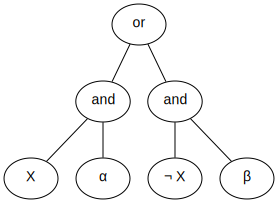
\includegraphics[width=\linewidth]{../thesis/gfx/bdd_lang.pdf}
        \caption[Sentence in BDD.]{Sentence in BDD.}
        \label{fig:bdd_lang}
    \end{subfigure} \quad
    \begin{subfigure}[b]{.45\linewidth}
        \centering
        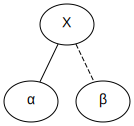
\includegraphics[width=\linewidth]{../thesis/gfx/bdd_data.pdf}
        \caption[BDD for the sentence in Figure \ref{fig:bdd_lang}.]{BDD for the sentence in Figure \ref{fig:bdd_lang}.}
        \label{fig:bdd_data}
    \end{subfigure}
    \caption[BDD]{Example of the same Boolean function represented
    as an NNF structure adhering to the BDD language
    constraints (Figure \ref{fig:bdd_lang}) and as the corresponding
    canonical BDD data structure (Figure \ref{fig:bdd_data}).}
    \label{fig:bdd}
\end{figure}

There are two subsets of BDss that are particularly
important: the Free Binary Decision Diagrams (FBDDs) and the
Ordered Binary Decision Diagrams (OBDDs). The former has a
property called \textit{read-once}, which means that for each
path from the root to a leaf, each variable appears at most
once. The latter has a property called \textit{ordering}, which
enables it to have canonical representations. In this context,
the order of the variables is fixed and consistent for all
OBDDs that represent the same function. This property also
enables operations such as \textit{conjunction} and
\textit{disjunction}, making it possible to construct OBDDs
from the bottom up by applying these operations
\citep{akers1978binary, bryant1986graph}.

\begin{definition}[Free Binary Decision Diagrams]
The FBDD language is the subset of the BDD
language that intersects with the DNNF language.
\end{definition}

\begin{remark}
By constraining a BDD to follow the
\textbf{decomposability} property, one obtains the
\textbf{read-once} property, as mentioned earlier.
\end{remark}

\begin{definition}[Ordered Binary Decision Diagrams]
The OBDD language is the subset of the FBDD
language that follows the \textbf{order} property.
\end{definition}

\begin{remark}
By constraining an FBDD to follow the \textbf{order}
property, one enables the use of the \textbf{apply}
operation and many other efficient algorithms to manipulate
OBDDs \citep{bryant1986graph}.
\end{remark}

Although they are no longer considered state-of-the-art in
Circuit Theory for succinctly representing Boolean formulas, their
historical importance, combined with the possibility of
bottom-up construction, still makes BDDs a relevant topic.
In particular, this language had a significant influence on the
development of SDDs, a subset of DNNFs that enables
bottom-up construction and efficient algorithms for performing
a diverse range of logical queries \citep{darwiche2011sdd}.

\section{Sentential Decision Diagrams}

Sentential Decision Diagrams are a subset of DNNFs that
aim to achieve the succinctness of more general d-DNNF, which
are capable of reasoning over a diverse range of probabilistic
applications, while still allowing for bottom-up construction
and efficient operations \citep{darwiche2011sdd}. Another
desirable property that SDDs aim to achieve is
\textit{canonicity}, which allows OBDDs to optimize their
succinctness by searching for the best variable ordering (instead of
a process of searching for an optimal compilation)
\citep{darwiche2011sdd}.

To define this language, we need to introduce two
new properties: \textit{structured decomposability} and
\textit{strong determinism}, both generalizations of the
homonymous properties described in \autoref{sec:nested}.

It is worth noting that these two concepts, \textit{structured
decomposability} and \textit{strong determinism}, are based on
generalizations of \textit{variable ordering} and
\textit{Shannon decomposition}, respectively, which are both
used in OBDDs to achieve canonicity and succinctness. These
generalizations are referred to as \textit{v-trees}
and \textit{strong deterministic decompositions}, respectively
\citep{darwiche2011sdd}.

Moreover, by introducing weaker constraints than OBDDs,
SDDs are capable of achieving more succinct representations
than OBDDs, while still preserving canonicity and allowing
for efficient algorithms to perform Boolean operations
\citep{darwiche2011sdd}.


\subsection{Structured Decomposability}

Before introducing the set of constraints that enable a more
structured version of d-DNNF, by requiring a structured
version of the decomposability property, we need to introduce
the concept of \textit{v-trees}, as follows:

\begin{definition}[V-tree]
A \textit{v-tree} for a set of variables $V$ is a full rooted
binary tree whose leaves are in one-to-one
correspondence with the variables in $V$.

For a node $n$ in a \textit{v-tree} $T$, we define
$\mathrm{vars}(n)$ as the set of variables in the leaves of
the subtree rooted at $n$. Moreover, for each non-leaf node
$n$, we define $n^l$ and $n^r$ as the left and right children
of $n$, respectively.

Lastly, if $V$ includes the variables of a formula $\Delta$,
we say that $T$ is a \textit{v-tree} for $\Delta$.
\end{definition}

\begin{definition}[DNNF w.r.t. a V-tree]
We say that a DNNF $\Sigma$ respects a \textit{v-tree}
$T$ if, for each conjunction $\alpha \land \beta$ in
$\Sigma$, there is a node $n$ in $T$ such that
$\mathrm{vars}(\alpha) \subseteq \mathrm{vars}(n^l)$ and
$\mathrm{vars}(\beta) \subseteq \mathrm{vars}(n^r)$.

The \textit{decomposition node} (\textit{d-node}) of a
sub-formula $\gamma$ of $\Sigma$ is defined as the deepest
node $n$ in $T$ such that $\mathrm{vars}(\gamma) \subseteq
\mathrm{vars}(n)$.
\end{definition}

With the two previous definitions, we can now define the subset
of DNNFs that respects a \textit{v-tree} $T$:

\begin{definition}[Smooth Decomposable NNF (SDNNF)]
We denote the set of all DNNFs that respect a
\textit{v-tree} $T$ as $\mathrm{DNNF}_T$. Moreover, we
define SDNNF as the set containing all
$\mathrm{DNNF}_T$, for any \textit{v-tree} $T$.
\end{definition}

\begin{example}
Figure \ref{fig:v-tree_and_dnnf} depicts a \textit{v-tree}
$T$ for variables $V = \{a, b, c, d, e\}$ and a
$\mathrm{DNNF}_T$ $\Sigma$.

\begin{figure}[bth]
    \centering
    \begin{subfigure}[b]{.45\linewidth}
        \centering
        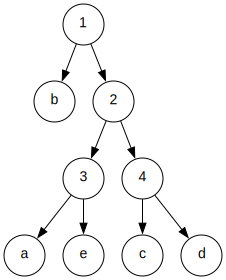
\includegraphics[width=\linewidth]{../thesis/gfx/vtree.pdf}
        \caption[A V-tree $T$ with all internal nodes labeled
        with their indices.]{A V-tree $T$ with all internal nodes labeled
        with their indices.}
        \label{fig:v-tree}
    \end{subfigure} \quad
    \begin{subfigure}[b]{.45\linewidth}
        \centering
        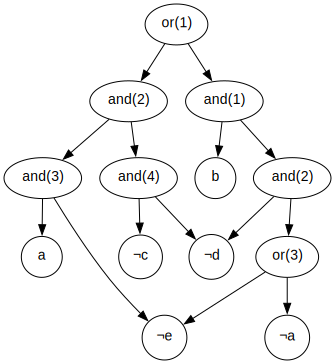
\includegraphics[width=\linewidth]{../thesis/gfx/dnnf_t_vtree.pdf}
        \caption[A \textit{structured} DNNF formula for
        $(\neg a \lor \neg e) \land (a \lor b) \land (b \lor
        \neg c) \land (c \lor \neg d) \lor (\neg b \land \neg
        d)$.]{A \textit{structured} DNNF formula for
        $(\neg a \lor \neg e) \land (a \lor b) \land (b \lor
        \neg c) \land (c \lor \neg d) \lor (\neg b \land \neg
        d)$.}
        \label{fig:dnnf_v-tree}
    \end{subfigure}
    \caption[V-tree and structured BDD]{A V-tree $T$
    (Figure \ref{fig:v-tree}) and a DNNF $\Sigma$
    (Figure \ref{fig:dnnf_v-tree}) that respects $T$. Each
    internal node of $\Sigma$ is labeled with the index of
    its decomposition node (d-node) in $T$
    \citep{pipatsrisawat2008new}.}
    \label{fig:v-tree_and_dnnf}
\end{figure}
\end{example}

The most interesting property of SDNNF is that it allows
the application of the polynomial-time \textit{Conjoin} operator
\citep{pipatsrisawat2008new}. More specifically, given two
DNNFs $\Sigma_1$ and $\Sigma_2$ that respect the same
V-tree $T$, the \textit{Conjoin} operator constructs a new
$\mathrm{DNNF}_T$ $\Sigma$ that represents the conjunction
$\alpha \land \beta$ of the formulas represented by $\Sigma_1$
and $\Sigma_2$; and this operation can be performed in polynomial
time with respect to the product of the sizes of $\Sigma_1$ and
$\Sigma_2$.

\subsection{Strong Determinism}

When defining \textit{strong determinism}, we must also introduce a fundamental
concept for this property, referred to as an $(X,Y)$-decomposition of a Boolean
function $f$. This decomposition allows $f$ to be expressed in terms of
functions on $X$ and $Y$ \citep{darwiche2011sdd}.

\begin{definition}[$(X,Y)$-Decomposition]
Let $f$ be a Boolean function of the form $f = (p_1(X)
\land s_1(Y)) \lor \ldots \lor (p_k(X) \land s_k(Y))$. Then,
$f$ has an $(X,Y)$-decomposition $\set{(p_1,s_1), \ldots,
(p_k,s_k)}$. Each ordered pair $(p_i, s_i)$ is called an
\textit{element} of the decomposition, and both $p_i$ and
$s_i$ are referred to as \textit{prime} and \textit{sub},
respectively.

The size of a decomposition is defined as the number of its elements.

Furthermore, if $p_i \land p_j = \mathit{false}$ for all $i
\ne j$, then the decomposition is said to be
\textit{strongly deterministic} on $X$.
\end{definition}

Sentential Decision
Diagramsare a proper subset of SDNNFs that adhere to a more structured
decomposition \citep{darwiche2011sdd}, defined as follows:

\begin{definition}[$X$-partition]
Let $\alpha = \set{(p_1, s_1), \ldots, (p_k, s_k)}$ be an
$(X,Y)$-decomposition of a Boolean function $f$, such that
this decomposition is strongly deterministic on $X$. Then,
$\alpha$ is called an $X$-partition of $f$ if and only if
its primes form a partition. Specifically, the primes of
$\alpha$ are consistent, mutually exclusive, and the
disjunction of all primes is valid.

Moreover, $\alpha$ is said to be \textit{compressed} if and
only if its subs are all distinct.
\end{definition}

These types of partitions exhibit some interesting properties. For
example, one can always convert an uncompressed partition into
a compressed one by replacing elements $(p,s)$ and $(q,s)$ with
$(p \lor q, s)$, which does not alter the function represented.
Furthermore, it is clear by definition that \textit{false} can
never be a prime of an $X$-partition; and if \textit{true} is
a prime, then it is the only prime. Lastly, \textbf{primes
determine subs}. Hence, primes of different $X$-partitions of
the same function $f$ must form different partitions
\citep{darwiche2011sdd}.

A more notable observation is that OBDDs are
based on the following $X$-partition of a function $f$: $\set{(X,
f \mid X), (\neg X, f \mid \neg X)}$, where $f \mid X$ is the
result of \textit{conditioning} $f$ on $X$
\citep{darwiche2011sdd}. This specific decomposition is called
a \textbf{Shannon decomposition}, and the \textit{decisions}
of OBDDs are binary, as they are based on the
value of literal primes $X$ and $\neg X$.

The main idea behind SDDs is to generalize this concept,
where the decisions are not binary because $X$ corresponds to a
set of variables instead of a single variable. In this way, the
decisions are based on the values of sentential primes
\citep{darwiche2011sdd}.

\subsection{Formal Definition}

As mentioned earlier, SDDs are a proper subset of
SDNNFs, structured decomposable NNFs, that also
respect strong determinism via (compressed) $X$-partitions.

\begin{definition}[Sentential Decision Diagrams (SDDs)]
We say that $\alpha$ is an SDD that respects a v-tree
$T$ rooted at $v$ if and only if:
\begin{itemize}
    \item $\alpha = \top$ or $\alpha = \bot$;
    \item $\alpha = X$ or $\alpha = \neg X$, and $T$ is a
    leaf labeled with $X$; or
    \item $\alpha = \set{(p_1, s_1), \ldots, (p_k, s_k)}$,
    $v$ is an internal node, $p_1, \ldots, p_k$ are
    SDDs that respect subtrees of $v^l$, and $s_1,
    \ldots, s_k$ are SDDs that respect subtrees of
    $v^r$, and $\braket{p_1}, \ldots, \braket{p_k}$ is a
    partition,
\end{itemize}

where $\braket{p}$ denotes a mapping from SDDs into
Boolean functions.

In the third case, if the primes of $\alpha$
respect $v^l$ and the subs respect $v^r$ (instead of
respecting the subtrees $v^l$ and $v^r$), then the SDD
$\alpha$ is said to be \textit{normalized}.

The semantics of an SDD $\alpha$ is defined,
with respect to the items above, as follows:
\begin{itemize}
    \item $\braket{\top} = \mathit{true}$ and $\braket{\bot}
    = \mathit{false}$;
    \item $\braket{X} = X$ and $\braket{\neg X} = \neg X$;
    \item $\braket{\alpha} = \bigvee_{i=1}^k \braket{p_i}
    \land \braket{s_i}$.
\end{itemize}

Finally, the size of an SDD $\alpha$ is denoted by
$|\alpha|$ and is the sum of the sizes of all its
decompositions.
\end{definition}

\begin{example}
Figure \ref{fig:sdd_darwiche} shows an example of an
SDD, but using a different notation than the one that
is typically used. In this case, the notation of the SDD
follows the NNF language, aiming to present this
structure in a unified framework.

\begin{figure}[bth]
    \centering
    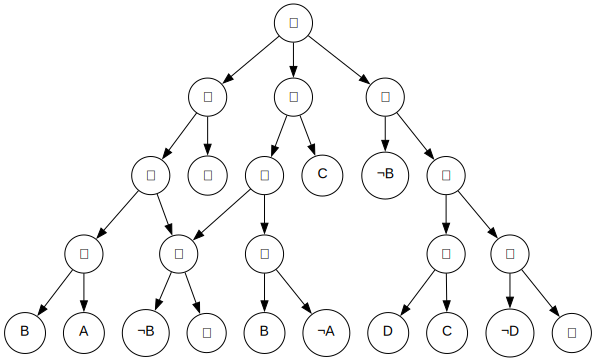
\includegraphics[width=0.95\textwidth]{../thesis/gfx/sdd_darwiche.pdf}
    \caption[SDD]{A SDD (in NNF)
    representing a Boolean function $f = (A \land B) \lor (B
    \land C) \lor (C \land D)$, following the variable order
    $\braket{B, A, C, D}$, with the V-tree described in more
    detail in \citep{darwiche2011sdd}.}
    \label{fig:sdd_darwiche}
\end{figure}
\end{example}

One last important property of SDDs concerns their
canonicity. More specifically, if two SDDs $\alpha$ and
$\beta$ are both compressed and trimmed (with the definitions of
these properties as follows), respecting nodes in the same
V-tree, then they represent the same Boolean function if and
only if they are equal \citep{darwiche2011sdd}.

\begin{definition}[Compressed and Trimmed SDDs]
We say that an SDD $\alpha$ is \textit{compressed} if
and only if, for all decompositions $\set{(p_1, s_1),
\ldots, (p_k, s_k)}$ of $\alpha$, all subs are
pairwise inequivalent ($s_i \not \equiv s_j$, when $i \ne
j$). Moreover, we say that $\alpha$ is \textit{trimmed} if
and only if it does not have any decompositions of the form
$\set{(\top, \beta)}$ or $\set{(\beta, \top), (\neg \beta,
\bot)}$.
\end{definition}

\subsection{SDD Operations}

The importance of the properties defined above is not only related
to \textit{canonicity} but also to the efficient computation of
Boolean functions. By imposing the \textit{trimming} and
\textit{compression} properties, it is possible to assert that:

\begin{enumerate}[label=(\roman*), ref=\roman*]
\item Trivial SDDs $\bot$ and $\top$ are the only ones
capable of representing the trivial Boolean functions,
$\mathit{false}$ and $\mathit{true}$, respectively;
\item Non-trivial SDDs respect unique \textit{V-tree}
nodes, which depend on the functions they represent.
\end{enumerate}

Another way to support this assertion is by imposing the
\textit{compression}, \textit{light trimming}, and
\textit{normalization} properties, where \textit{light trimming}
corresponds to the exclusion of decompositions of the form
$\set{\top, \top}$ or $\set{\top, \bot}$ by replacing them with
$\top$ and $\bot$, respectively \citep{darwiche2011sdd}.

By ensuring these three properties, it is possible to
support the claim that a Boolean function $f$ can be uniquely
represented by an SDD, given a fixed V-tree $T$.

Moreover, two normalized and lightly trimmed SDDs for
the same V-tree, say $\alpha$ and $\beta$, can perform
the application of any binary operator $\circ$,
resulting in $\braket{\alpha} \circ \braket{\beta}$, in
polynomial time $O(|\alpha| \cdot |\beta|)$, by following
the \textit{Apply} operator described in \citep{darwiche2011sdd}.
This SDD \textit{Apply} algorithm closely resembles the algorithm
for the \textit{Apply} operator in BDDs \citep{bryant1986graph},
with the key difference being the use of $V$-trees instead of
variable orderings.

% \begin{algorithm}
% \caption{Sentential Decision Diagram Apply Algorithm}
% \label{alg:apply}
% \begin{algorithmic}[1]
%     \Require A tuple \(\alpha, \beta, \circ\), formed by
%     \begin{enumerate}[label=(\roman*),ref=\roman*]
%         \item an SDD \(\alpha\), that is lightly
%         trimmed and normalized for a \textit{v-tree} \(T\),
%         \item an SDD \(\beta\), that is also lightly
%         trimmed and normalized for \(T\), and
%         \item a Boolean operator \(\circ\).
%     \end{enumerate}
%     %
%     \Ensure An SDD $\Delta$ that is lightly trimmed,
%     normalized for \(T\), and represents the function
%     \(\braket{\alpha} \circ \braket{\beta}\).
%     \vspace{4pt}
%     \hrule
%     \vspace{4pt}
%     \(\textsc{Cache}(\_,\_,\_) = \textsc{nil}\) initially.
%     \(\textsc{Expand}(\gamma)\) returns \(\set{\top, \top}\)
%     if \(\gamma = \top\); \(\set{\top, \bot}\) if \(\gamma =
%     \bot\); and \(\gamma\) otherwise. \(\textsc{UniqueD}(
%     \gamma)\) returns \(\top\) if \(\gamma = \set{\top,\top}
%     \); \(\bot\) if \(\gamma = \set{\top,\bot}\); and the
%     unique SDD with elements \(\gamma\) otherwise.
%     \vspace{4pt}
%     \hrule
%     \vspace{4pt}
%     %
%     \Function{SDD-Apply}{$\alpha, \beta, \circ$}
%     %
%     \If {\(\alpha\) and \(\beta\) are \textbf{constants} or
%     \textbf{literals}}
%     %
%         \State \textbf{return} \(\alpha \circ \beta\)
%     %
%     \ElsIf {\(\textsc{Cache}(\alpha, \beta, \circ) \ne \textsc{nil}\)}
%     %
%         \State \textbf{return} \(\textsc{Cache}(\alpha, \beta, \circ)\)
%     %
%     \EndIf
%     %
%     \State \(\gamma \gets \set{}\)
%     %
%     \ForAll {\((p_i, s_i) \in \textsc{Expand}(\alpha)\)}
%     %
%         \ForAll {\((q_j, r_j) \in \textsc{Expand}(\beta)\)}
%     %
%             \State \(p \gets \textsc{SDD-Apply}(p_i, q_j, \land)\)
%     %
%             \If {\(p\) is \textbf{consistent}}
%     %
%                 \State \(s \gets \textsc{Apply}(s_i, r_j, \circ)\)
%     %
%                 \State add element \((p,s)\) to \(\gamma\)
%     %
%             \EndIf
%     %
%         \EndFor
%     %
%     \EndFor
%     %
%     \State \textbf{return} \(\textsc{Cache}(\alpha, \beta,
%     \circ) \gets \textsc{UniqueD}(\gamma)\)
%     %
%     \EndFunction
% \end{algorithmic}
% \end{algorithm}

\begin{example}
Figure \ref{fig:sdd_apply} illustrates a \textit{conjoin}
operation between two SDDs $\alpha$ and $\beta$, each
representing $A \land B$ and $\neg A \lor \neg C$, following
a balanced V-tree $T$.

\begin{figure}[bth]
    \centering
    \begin{subfigure}[b]{.28\linewidth}
        \centering
        \includegraphics[height=5cm]{../thesis/gfx/sdd_apply1.pdf}
        \caption[An SDD $\alpha$ representing $A \land B$.]{An SDD $\alpha$ representing $A \land B$.}
        \label{fig:sdd_apply_left}
    \end{subfigure} \quad
    \begin{subfigure}[b]{.28\linewidth}
        \centering
        \includegraphics[height=5cm]{../thesis/gfx/sdd_apply2.pdf}
        \caption[An SDD $\beta$ representing $\neg A \lor \neg C$.]{An SDD $\beta$ representing $\neg A \lor \neg C$.}
        \label{fig:sdd_apply_right}
    \end{subfigure} \quad
    \begin{subfigure}[b]{.28\linewidth}
        \centering
        \includegraphics[height=5cm]{../thesis/gfx/sdd_apply.pdf}
        \caption[The result of the \textit{conjoin} operation between $\alpha$ and $\beta$.]{The result of the \textit{conjoin} operation between $\alpha$ and $\beta$.}
        \label{fig:sdd_apply_result}
    \end{subfigure}
    \caption[SDD Apply Operation]{Two SDDs
    $\alpha$ and $\beta$ (Figures \ref{fig:sdd_apply_left}
    and \ref{fig:sdd_apply_right}, respectively) and the
    result of the \textit{conjoin} operation between them
    (Figure \ref{fig:sdd_apply_result}).}
    \label{fig:sdd_apply}
\end{figure}
\end{example}

\subsubsection{Comparison between SDDs and BDss}

The two main characteristic properties of OBDDs are their
canonicity and efficient computation of Boolean functions such
as \textit{conjunction}, \textit{disjunction}, and
\textit{negation}. As mentioned earlier, the imposition
of \textit{structured decomposability} enables one to perform
a polynomial-time \textit{conjoin} operation, whereas the
\textit{strong determinism} property (together with
\textit{partitioning}) enables one to perform the
\textit{disjoin} binary Boolean operation in polynomial time,
retrieving a new SDD that represents the disjunction
of two functions represented by two SDDs
\citep{darwiche2011sdd}. Furthermore, SDDs are also capable
of performing the \textit{negation} operation in polynomial time,
which enables their use in a wide range of applications that
OBDDs are used for
\citep{darwiche2011sdd, Darwiche_2002}.

On the other hand, \textit{compressed} and
\textit{trimmed} SDDs ensure the \textit{canonicity}
property, similar to OBDDs.

As stated at the start of this section, SDDs are a
proper subset of SDNNF, which are a proper subset of
DNNF \citep{pipatsrisawat2008new}. Another interesting
relation is that OBDDs are a subset of SDDs, where the
corresponding V-trees are \textit{right-linear}, i.e., each
left child is a leaf \citep{darwiche2011sdd}. Both of these
relations together render the following hierarchy of
succinctness:
\begin{equation}
\mathrm{OBDD} \le \mathrm{SDD} < \mathrm{d\text{-}DNNF},
\label{eq:succinctness_hierarchy}
\end{equation}
where all of these languages are capable of efficiently
performing \textit{model counting} inferences
\citep{Darwiche_2002}; whereas d-DNNF are only capable of
performing \textit{conjunction} and \textit{disjunction}
operations if $P = NP$ \citep{Darwiche_2002}.

%\subsection{Probabilistic Sentential Decision Diagrams}
%
%A more recent proposal, related to the field of tractable
%Probabilistic Reasoning, is the \ac{PSDD} language, which is an
%extension of the SDD language that allows for the
%canonical representation of probability distributions defined
%over models of a given propositional theory
%\citep{kisa2014probabilistic}.
%
%The main idea behind \acp{PSDD} is that each parameter of its
%structure can be interpreted as the conditional probability of a
%decision in a corresponding SDD. More specifically, we
%define \acp{PSDD} and their semantics as follows
%\citep{kisa2014probabilistic}:
%
%\begin{definition}[\acl{PSDD}]
%A \ac{PSDD} is an extension of a \textit{normalized}
%SDD with the following parameters:
%\begin{itemize}
%    \item For each terminal node $\top$, a positive
%    parameter $\theta$ is associated, such that $0 < \theta
%    < 1$; or
%    \item For each decision node $(p_1, s_1), \ldots, (p_k,
%    s_k)$ and a prime $p_i$, a positive parameter $\theta_i$
%    is associated such that the set of parameters $\Theta =
%    \set{\theta_1, \ldots, \theta_k}$ is a convex
%    combination, and $\theta_i$ is positive if and only if
%    $s_i \ne \bot$.
%\end{itemize}
%\end{definition}
%
%\begin{definition}[\ac{PSDD} Distribution]
%Let $n$ be a node of a \ac{PSDD} $\alpha$ that is normalized
%for a V-tree node $v$. Then, we have that node $n$ defines a
%distribution $\mathbb{P}_n$ over the variables of $v$ as
%follows:
%\begin{itemize}
%    \item If $n$ is a terminal node and $v$ has variable
%    $X$, then
%    \begin{table}[ht!]
%        \begin{center}
%            \begin{tabular}[c]{r|c c}
%                $n$ & $\mathbb{P}_n(X)$ & $\mathbb{P}_n(\neg X)$ \\
%                \hline
%                $X:\theta$ & $\theta$ & $1 - \theta$ \\
%                $\bot$ & $0$ & $0$ \\
%                $X$ & 1 & 0 \\
%                $\neg X$ & 0 & 1 \\
%            \end{tabular}
%        \end{center}
%    \end{table}
%
%where $X:\theta$ denotes a terminal node $\top$ with
%parameter $\theta$; or
%
%\item If $n$ is a decision node $(p_1, s_1, \theta_1),
%\ldots, (p_k, s_k, \theta_k)$ and $v$ has left variables
%$X$ and right variables $Y$, then
%$$\mathbb{P}_n(xy) \coloneqq \mathbb{P}_{p_i}(x) \cdot
%\mathbb{P}_{s_i}(y) \cdot \theta_i, \quad \text{for $i$
%where $x \models p_i$}.$$
%\end{itemize}
%\end{definition}
%
%\begin{definition}[Parameter Semantics]
%Let $n$ be a \ac{PSDD} decision node $(p_1, s_1, \theta_1),
%\ldots, (p_k, s_k, \theta_k)$. Then, we have that $\theta_i
%= \mathbb{P}_n([p_i])$, where $[p_i]$ is the SDD node
%associated with the \ac{PSDD} node $p_i$.
%\end{definition}
%
%Note that, since we are considering an extension of SDDs,
%we are able to perform \acl{WMC} queries in polynomial time.
%Furthermore, a large range of probabilistic queries can be
%executed efficiently with \acp{PSDD}, besides the possibility
%of learning its parameters, as shown in \citep{kisa2014probabilistic}.

%------------------------------------------------
